\documentclass[a4paper,12pt]{book}
\usepackage[utf8]{inputenc}
\usepackage[top=2.54cm, bottom=2.54cm, left=2.54cm, right=2.54cm]{geometry}
\usepackage{graphicx}
\usepackage{pdfpages}
\usepackage{titlesec}
\usepackage{fancyhdr}
\usepackage{emptypage}
\usepackage{setspace}
\usepackage{indentfirst}
\usepackage{parskip}
\usepackage{fontspec}
\usepackage{booktabs}
\usepackage{enumitem}
\usepackage{multicol}
\usepackage{ragged2e}
\usepackage{hyphenat}
\usepackage{lettrine}
\usepackage{epigraph}
\usepackage{bookmark}

% Türkçe karakter desteği
\setmainfont{Times New Roman}
\setsansfont{Arial}

% Satır aralığı ayarı
\onehalfspacing

% Paragraf girintisi
\setlength{\parindent}{1.5em}

% Sayfa numaraları için ayarlar
\pagestyle{fancy}
\fancyhf{}
\fancyhead[LE]{\leftmark}
\fancyhead[RO]{\rightmark}
\fancyfoot[LE,RO]{\thepage}
\renewcommand{\headrulewidth}{0.4pt}
\renewcommand{\footrulewidth}{0.4pt}

% Bölüm başlıkları için ayarlar
\titleformat{\chapter}[display]
{\normalfont\huge\bfseries}{\chaptertitlename\ \thechapter}{20pt}{\Huge}
\titlespacing*{\chapter}{0pt}{-50pt}{40pt}

% Alt bölüm başlıkları için ayarlar
\titleformat{\section}
{\normalfont\Large\bfseries}{\thesection}{1em}{}
\titlespacing*{\section}{0pt}{3.5ex plus 1ex minus .2ex}{2.3ex plus .2ex}

% Alt-alt bölüm başlıkları için ayarlar
\titleformat{\subsection}
{\normalfont\large\bfseries}{\thesubsection}{1em}{}
\titlespacing*{\subsection}{0pt}{2.3ex plus 1ex minus .2ex}{1.5ex plus .2ex}

% Boş sayfalar için ayarlar
\makeatletter
\renewcommand{\cleardoublepage}{\clearpage\if@twoside \ifodd\c@page\else
    \hbox{}\thispagestyle{empty}\newpage\if@twocolumn\hbox{}\newpage\fi\fi\fi}
\makeatother

% İçindekiler ayarları
\renewcommand{\contentsname}{İÇİNDEKİLER}
\renewcommand{\chaptername}{BÖLÜM}
\renewcommand{\appendixname}{EK}

\begin{document}

% Dış kapak
\begin{titlepage}
\begin{center}
\vspace*{2cm}
{\Huge\bfseries KORUYUCU AYETLER VE ŞİFA DUALARI\par}
\vspace{1cm}
{\Large\bfseries İslami Kaynaklardan Derlenmiş\par}
\vspace{2cm}

{\large Hazırlayan:\\[Yazar Adı]\par}
\vspace{1cm}
{\large \today\par}
\end{center}
\end{titlepage}

% İç kapak
\begin{titlepage}
\begin{center}
\vspace*{2cm}
{\Huge\bfseries KORUYUCU AYETLER VE ŞİFA DUALARI\par}
\vspace{1cm}
{\Large\bfseries İslami Kaynaklardan Derlenmiş\par}
\vspace{2cm}

{\large Hazırlayan:\\[Yazar Adı]\par}
\vspace{1cm}
{\large \today\par}
\end{center}
\end{titlepage}

% Telif hakkı sayfası
\begin{titlepage}
\begin{center}
\vspace*{2cm}
{\large © 2024 Tüm hakları saklıdır.\par}
\vspace{1cm}
{\large ISBN: [ISBN Numarası]\par}
\vspace{1cm}
{\large Baskı: [Baskı Sayısı]\par}
\vspace{1cm}
{\large Yayıncı: [Yayınevi Adı]\par}
\end{center}
\end{titlepage}

% İçindekiler
\tableofcontents
\cleardoublepage

% Ana içerik
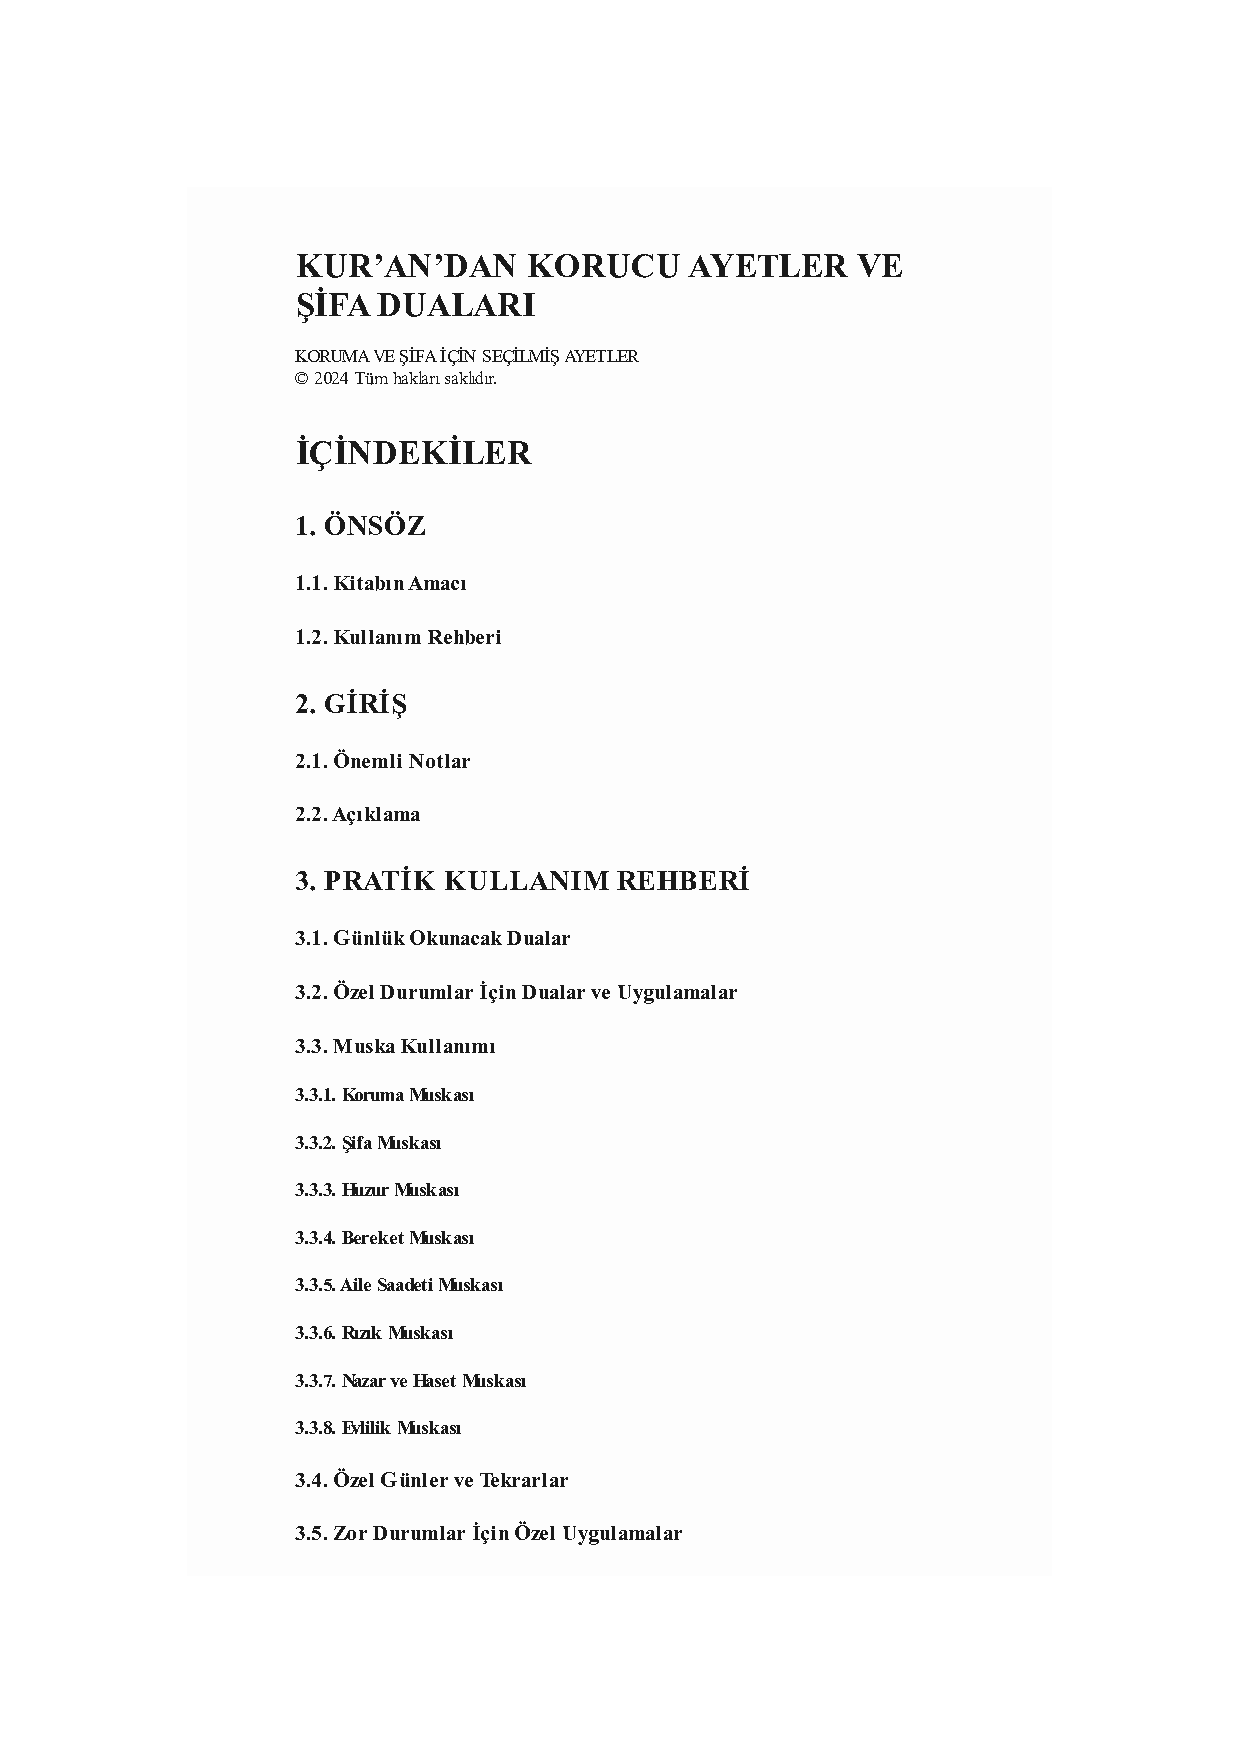
\includepdf[pages=-]{output/kitap.pdf}

% Kaynakça
\chapter{KAYNAKÇA}
\addcontentsline{toc}{chapter}{KAYNAKÇA}
\markboth{KAYNAKÇA}{KAYNAKÇA}

% Kaynakça içeriği buraya eklenecek

\end{document} 